\let\negmedspace\undefined
\let\negthickspace\undefined
\documentclass[journal]{IEEEtran}
\usepackage[a5paper, margin=10mm, onecolumn]{geometry}
%\usepackage{lmodern} % Ensure lmodern is loaded for pdflatex
\usepackage{tfrupee} % Include tfrupee package

\setlength{\headheight}{1cm} % Set the height of the header box
\setlength{\headsep}{0mm}     % Set the distance between the header box and the top of the text

\usepackage{gvv-book}
\usepackage{gvv}
\usepackage{cite}
\usepackage{amsmath,amssymb,amsfonts,amsthm}
\usepackage{algorithmic}
\usepackage{graphicx}
\usepackage{textcomp}
\usepackage{xcolor}
\usepackage{txfonts}
\usepackage{listings}
\usepackage{enumitem}
\usepackage{mathtools}
\usepackage{gensymb}
\usepackage{comment}
\usepackage[breaklinks=true]{hyperref}
\usepackage{tkz-euclide} 
\usepackage{listings}
% \usepackage{gvv}                                        
\def\inputGnumericTable{}                                 
\usepackage[latin1]{inputenc}                                
\usepackage{color}                                            
\usepackage{array}                                            
\usepackage{longtable}                                       
\usepackage{calc}                                             
\usepackage{multirow}                                         
\usepackage{hhline}                                           
\usepackage{ifthen}                                           
\usepackage{lscape}
\usepackage{circuitikz}


\renewcommand{\thefigure}{\theenumi}
\renewcommand{\thetable}{\theenumi}
\setlength{\intextsep}{10pt} % Space between text and floats


\numberwithin{equation}{enumi}
\numberwithin{figure}{enumi}
\renewcommand{\thetable}{\theenumi}


% Marks the beginning of the document
\begin{document}
\bibliographystyle{IEEEtran}
\vspace{3cm}

\title{GATE ASSIGNMENTS -1}
\author{EE25BTECH11028 - J.Navya Sri}
\date{}
\maketitle

\noindent
Q.1 -- Q.20 carry one mark each.

\begin{enumerate}
\item If $A$ is an orthogonal matrix, then
\hfill(MN.2009)

\begin{enumerate}[label=(\Alph*)]
\begin{multicols}{4}
\item $A^T = A^{-1}$
\item $A^T = -A^{-1}$
\item $A = A^{-1}$
\item $A = -A^{-1}$
\end{multicols}
\end{enumerate}

\item In a normal (Gaussian) distribution curve, the area between one standard deviation from mean on either side in percent is
\hfill{(MN.2009)}
\begin{enumerate}[label=(\Alph*)]
\begin{multicols}{4}
    \item $50$
    \item $68$
    \item $86$
    \item $95$
 \end{multicols}
\end{enumerate}

\item A measure of dispersion of a sample data set is
\hfill{(MN.2009)}
\begin{enumerate}[label=(\Alph*)]
   \begin{multicols}{4}
    \item mean
    \item median
    \item mode
    \item standard deviation
 \end{multicols}
\end{enumerate}

\item The value of $\displaystyle \lim_{x \to 2} \left(\frac{2\sqrt{4-x^2}}{5}\right)$ is
\hfill{(MN.2009)}
\begin{enumerate}[label=(\Alph*)]
  \begin{multicols}{4}
    \item $-\frac{2\sqrt{8}}{5}$
    \item $0$
    \item $\frac{2\sqrt{8}}{5}$
    \item non-existent
     \end{multicols}
\end{enumerate}

\item $\hat{i}, \hat{j}$ and $\hat{k}$ represent the unit vectors in the positive $x, y$ and $z$ directions of a Cartesian coordinate system. Using the right-hand rule, $\hat{k} \times \hat{j}$ represents
\hfill{(MN.2009)}
\begin{enumerate}[label=(\Alph*)]
   \begin{multicols}{4}
 \item $0$
    \item $1$
    \item $-\hat{i}$
    \item $\hat{i}$
     \end{multicols}
\end{enumerate}

\item The rock mass classification system that considers ``active stress" factor is
\hfill{(MN.2009)}
\begin{enumerate}[label=(\Alph*)]
  \begin{multicols}{4}
    \item Q-system
    \item RMR
    \item RQD
    \item GSI
         \end{multicols}
\end{enumerate}

\item In a triaxial compression test if $\sigma_1$ is axial stress and $\sigma_2$ and $\sigma_3$ are confining stresses, then
\hfill{(MN.2009)}
\begin{enumerate}[label=(\Alph*)]
 \begin{multicols}{4}
    \item $\sigma_3 > \sigma_2 = \sigma_1$
    \item $\sigma_1 > \sigma_2 = \sigma_3$
    \item $\sigma_1 = \sigma_2 > \sigma_3$
    \item $\sigma_3 = \sigma_2 > \sigma_1$
       \end{multicols}
\end{enumerate}

\item In a longwall mining subsidence phenomenon, the ``angle of break" is the angle between
\hfill{(MN.2009)}
\begin{enumerate}[label=(\Alph*)]
    \item the vertical line at the panel edge and line connecting the panel edge and zero subsidence on the surface
    \item the vertical line at the panel edge and line connecting the panel edge and point of critical deformation on the surface
    \item the vertical line at the panel edge and line connecting the panel edge and the point of the maximum tensile strain on the surface
    \item the horizontal line and the line connecting the panel edge and zero subsidence on the surface
\end{enumerate}

\item The main advantage of single stage mining method over the two-stage mining method is
\hfill{(MN.2009)}
\begin{enumerate}[label=(\Alph*)]
\begin{multicols}{4}
 \item higher recovery of coal
    \item better roof control
    \item increased safety
    \item lower cost
    \end{multicols}
\end{enumerate}

\item The maximum dip angle of a coal seam for mechanized mining is
\hfill{(MN.2009)}
\begin{enumerate}[label=(\Alph*)]
    \item 15\degree
    \item 25\degree
    \item 30\degree
    \item 45\degree
\end{enumerate}

\item The primary purpose of a ventilation system in an underground mine is to
\hfill{(MN.2009)}
\begin{enumerate}[label=(\Alph*)]
    \item remove harmful gases and provide fresh air
    \item reduce the temperature of the mine
    \item prevent water accumulation
    \item control dust levels
\end{enumerate}

\item Which of the following is a method of mine ventilation?
\hfill{(MN.2009)}
\begin{enumerate}[label=(\Alph*)]
    \item Natural ventilation
    \item Mechanical ventilation
    \item Both (A) and (B)
    \item None of the above
\end{enumerate}

\item Shotcrete is mainly used in mines for
\hfill{(MN.2009)}
\begin{enumerate}[label=(\Alph*)]
    \item ground support
    \item ventilation
    \item drainage
    \item lighting
\end{enumerate}

\item In a mine survey, a theodolite is used to measure
\hfill{(MN.2009)}
\begin{enumerate}[label=(\Alph*)]
    \item distances
    \item angles
    \item elevations
    \item depths
\end{enumerate}

\item The electrical resistivity of a rock depends mainly on its
\hfill{(MN.2009)}
\begin{enumerate}[label=(\Alph*)]
    \item porosity and fluid content
    \item color and texture
    \item mineral composition
    \item temperature only
\end{enumerate}

\item In mine drainage, the most commonly used method for removing water is
\hfill{(MN.2009)}
\begin{enumerate}[label=(\Alph*)]
    \item pumping
    \item siphoning
    \item gravitational flow
    \item evaporation
\end{enumerate}

\item As per the DGMS norms, the severity index is a measure of
\hfill{(MN.2009)}
\begin{enumerate}[label=(\Alph*)]
    \item fatality rate
    \item serious injury rate
    \item number of reportable injuries
    \item accident proneness of mine
\end{enumerate}

\item A balanced transportation problem is characterized by
\hfill{(MN.2009)}
\begin{enumerate}[label=(\Alph*)]
    \item total supply exceeds total demand
    \item total demand exceeds total supply
    \item total demand is equal to total supply
    \item total supply is either equal to or more than total demand
\end{enumerate}

\item In the context of project management techniques, the TRUE statement is
\hfill{(MN.2009)}
\begin{enumerate}[label=(\Alph*)]
    \item CPM is stochastic and PERT is deterministic
    \item CPM is deterministic and PERT is stochastic
    \item Both CPM and PERT are deterministic
    \item Both CPM and PERT are stochastic
\end{enumerate}

\item For mining property appraisals, typical reports prepared are Bankable Feasibility Report (BFR), Conceptual Plan Report (CPR), Feasibility Report (FR) and Detailed Project Report (DPR). The chronological order for the preparation of these reports is
\hfill{(MN.2009)}
\begin{enumerate}[label=(\Alph*)]
    \item CPR $\to$ FR $\to$ BFR $\to$ DPR
    \item BFR $\to$ CPR $\to$ DPR $\to$ FR
    \item FR $\to$ BFR $\to$ CPR $\to$ DPR
    \item CPR $\to$ BFR $\to$ DPR $\to$ FR
\end{enumerate}

\item The mean of the cubes of the first $n$ natural numbers is
\hfill{(MN.2009)}
\begin{enumerate}[label=(\Alph*)]
    \item $\frac{n(n+1)^2}{4}$
    \item $\frac{n(n+1)(n+2)}{8}$
    \item $\frac{n^4 + 1}{n}$
    \item $\frac{n^3}{4}$
\end{enumerate}

\item The sum of the eigenvalues of the matrix 
\[\begin{bmatrix}1 & 2 \\1 & 0\end{bmatrix}\]is
\hfill{(MN.2009)}
\begin{enumerate}[label=(\Alph*)]
    \item $-3$
    \item $-1$
    \item $1$
    \item $3$
\end{enumerate}


    \item The value of $\nabla \cdot \mathbf{F}$ of a vector $\mathbf{F} = 4x^2 \hat{i} + 3xy^2 \hat{j} + xyz^2 \hat{k}$ at the point (1, 1, 2) is
    \hfill{(MN.2009)}
    \begin{enumerate}[label=(\Alph*)]
        \item $24$
        \item $26$
        \item $30$
        \item $32$
    \end{enumerate}

  \item The function $f(x) = x^2(1 - x)$ is integrated between 0 and 1 (both inclusive) using closed form method and also by Simpson's $\dfrac{1}{3}$ rule. ...
     The difference in the values obtained from these methods is
  \hfill{(MN.2009)}
    \begin{enumerate}[label=(\Alph*)]
        \item 0
        \item $\dfrac{1}{480}$
        \item $\dfrac{1}{120}$
        \item $\dfrac{1}{20}$
    \end{enumerate}

    \item Water starts to flow into a sump initially containing 250 kL of water. The inflow rate of water is $4t$ L/min where $t$ refers to time elapsed in min. If the pumping rate of water out of the sump is 250 L/min, the total volume of water in the sump after 3 hours in kL is
    \hfill{(MN.2009)}
    \begin{enumerate}[label=(\Alph*)]
        \item $250.5$
        \item $255.6$
        \item $269.8$
        \item $280.9$
    \end{enumerate}

    \item There are 50 lemon trees in a reclaimed mine area. Each tree produces 800 lemons per year. For each additional tree planted in this area, considering all trees, the output number of fruits per tree drops by 10 lemons in a year. The number of trees to be added to the existing reclaimed area in order to maximize the total number of lemons in the year is
    \hfill{(MN.2009)}
    \begin{enumerate}[label=(\Alph*)]
        \item $10$
        \item $15$
        \item $16$
        \item $26$
    \end{enumerate}

    \item The grain density and bulk density of a dry coarse grained sandstone rock sample are 3.0 gm/cc and 2.7 gm/cc respectively. The void ratio of the sample in percentage is
    \hfill{(MN.2009)}
    \begin{enumerate}[label=(\Alph*)]
        \item $8.4$
        \item $10.0$
        \item $11.1$
        \item $30.5$
    \end{enumerate}

    \item The ratio of uniaxial compressive strength to uniaxial tensile strength of a sandstone specimen is 8:1. The theoretical value of angle of internal friction of the specimen in degree is
    \hfill{(MN.2009)}
    \begin{enumerate}[label=(\Alph*)]
        \item $51$
        \item $41$
        \item $32$
        \item $7$
    \end{enumerate}

    \item A circular tunnel is made underground where far field vertical and horizontal stresses are $P_v$ and $KP_v$ respectively. The tangential stress ($\sigma_{\theta\theta}$) at the boundary of the tunnel for $\theta = 45^\circ$ from the horizontal plane is $3P_v$. The value of $K$ is
    \hfill{(MN.2009)}
    \begin{enumerate}[label=(\Alph*)]
        \item $0$
        \item $1$
        \item $2$
        \item $3$
    \end{enumerate}
    
\item The bending moment diagram for the shaft shown below resembles which one of the following graphs?
\hfill{(MN.2009)}
\begin{figure}[H]
    \centering
    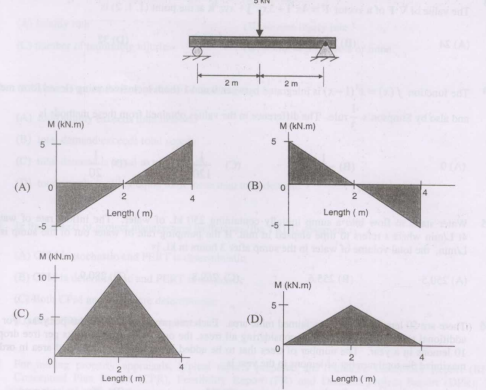
\includegraphics[width=0.5\linewidth]{figs/fig 3.png}
    \caption{graph}
    \label{fig:placeholder}
\end{figure}

    \item A mining equipment has a life of 5 years with no salvage value. Assuming that the depreciation of the equipment is calculated by the straight line method, the average annual value of the equipment in percentage of its original value is:
    \hfill{(MN.2009)}
    \begin{enumerate}
        \item $20$
        \item $40$
        \item $50$
        \item $60$
    \end{enumerate}

    \item Air flows at 2 m\textsuperscript{3}/s through a forcing fan duct of 0.3 m\textsuperscript{2} having uniform cross-section. The duct resistance is 40 Ns\textsuperscript{2}m\textsuperscript{-8} and air density is 1.2 kg/m\textsuperscript{3}. The total pressure generated by the fan in Pa is:
    \hfill{(MN.2009)}
    \begin{enumerate}
        \item $186.7$
        \item $160.0$
        \item $133.3$
        \item $26.7$
    \end{enumerate}

    \item Match the following in the context of Indian mining practice:
\hfill{(MN.2009)}
\begin{tabbing}
    \hspace{5cm} \= \textbf{Equipment} \hspace{6cm} \= \textbf{Power source} \kill
    \textbf{Equipment} \> \textbf{Power source} \\
    P. Rocker shovel \> 1. Battery \\
    Q. Locomotive \> 2. Compressed air \\
    R. Shearer \> 3. Electricity (maximum voltage 6.6 kV AC) \\
    S. Dragline (24 m\textsuperscript{3} bucket capacity) \> 4. Electricity (maximum voltage 1.1 kV AC) \\
    \end{tabbing}

    \begin{enumerate}
        \item P-1, Q-2, R-3, S-4
        \item P-2, Q-1, R-4, S-3
        \item P-2, Q-1, R-3, S-4
        \item P-1, Q-3, R-2, S-4
    \end{enumerate}

\item The planes H and V represent the horizontal and vertical planes respectively as shown in the figure. Which one of the following Mohr circles represents the stress conditions applied in planes H and V?

\begin{figure}[H]
\centering
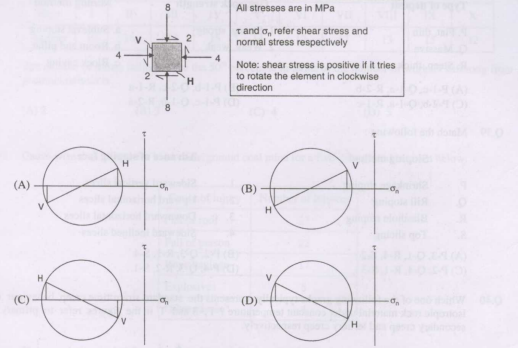
\includegraphics[width=0.4\columnwidth]{figs/fig2.png}
\caption{graph}
\label{fig:placeholder}
\end{figure}
\hfill{(MN.2009)}

\item Two splits A and B are ventilated from an intake airway. Resistances of the splits are $0.5 \, \text{Ns}^2/\text{m}^8$ and $0.8 \, \text{Ns}^2/\text{m}^8$ respectively. A regulator is placed in split B to maintain a flow of $15 \, \text{m}^3/\text{s}$ and $10 \, \text{m}^3/\text{s}$ in splits A and B respectively, as shown in the figure. The size of the regulator in $\text{m}^2$ is
\hfill{(MN.2009)}
\begin{figure}[H]
  \centering
  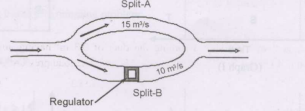
\includegraphics[width=0.4\columnwidth]{figs/fig1.png}
  \caption{Ventilation}
  \label{fig:placeholder}
\end{figure}


\begin{enumerate}[label=(\Alph*)]
    \item $2.10$
    \item $1.30$
    \item $1.20$
    \item $1.13$
\end{enumerate}

\item The concentration of OH$^-$ ion in a mine water sample is $10^{-11}$ mol/L. The pH of the sample is
\hfill{(MN.2009)}

\begin{enumerate}[label=(\Alph*)]
    \item $2$
    \item $3$
    \item $4$
    \item $11$
\end{enumerate}

\item A mine having a reserve of 320 Mt produces 4 Mt of ore at the end of 1\textsuperscript{st} year. If the mine increases production by 10\% every year, the percentage of the reserve that still remains at the end of 21\textsuperscript{st} year is
\hfill{(MN.2009)}
\begin{enumerate}[label=(\Alph*)]
    \item $50$
    \item $35$
    \item $25$
    \item $20$
\end{enumerate}

\item Match the following:
\hfill{(MN.2009)}
\begin{center}
\begin{tabular}{lll}
\textbf{Type of deposit} & \textbf{Ore, rock strength} & \textbf{Mining method} \\
P. Flat, thin & 1. Strong, strong & a. Sublevel stoping \\
Q. Massive & 2. Weak, weak & b. Room and pillar \\
R. Steep, thick & & c. Block caving \\
\end{tabular}
\end{center}

\begin{enumerate}[label=(\Alph*)]
\item P-1-c, Q-1-a, R-2-b
\item P-1-b, Q-2-c, R-1-a
\item P-2-b, Q-1-a, R-1-c
\item P-1-c, Q-1-b, R-2-a
\end{enumerate}

\item Match the following:
\hfill{(MN.2009)}
\begin{center}
\begin{tabular}{ll}
\textbf{Stoping method} & \textbf{Advance of stoping face} \\
P. Shrinkage stoping & 1. Sideward vertical slices \\
Q. Rill stoping & 2. Upward horizontal slices \\
R. Blasthole stoping & 3. Downward horizontal slices \\
S. Top slicing & 4. Sideward inclined slices \\
\end{tabular}
\end{center}

\begin{enumerate}[label=(\Alph*)]
\item P-3, Q-1, R-4, S-2
\item P-2, Q-3, R-1, S-4
\item P-2, Q-4, R-1, S-3
\item P-4, Q-3, R-2, S-1
\end{enumerate}

\item Which one of the following graphs typically represents the standard strain-time creep behaviour of an isotropic rock material under constant temperature? P, S and T in the figures refer to primary creep, secondary creep and tertiary creep respectively.
\hfill{(MN.2009)}
\begin{enumerate}[label=(\Alph*)]

\item
\begin{tikzpicture}[scale=1]
  % Axes
  \draw[->] (0,0) -- (5,0) node[right] {Time};
  \draw[->] (0,0) -- (0,3) node[above] {Strain};

  % Curves
  \draw[thick] plot [domain=0:4] (\x, {0.5*ln(\x+1)}) node[right] {};
  
  % Vertical dashed line for T
  \draw[dashed] (3,0) -- (3,2.2);
  
  % Points P, S, T on x-axis
  \node at (0,-0.3) {P};
  \node at (2,-0.3) {S};
  \node at (3,-0.3) {T};
\end{tikzpicture}

\item
\begin{tikzpicture}[scale=1]
  % Axes
  \draw[->] (0,0) -- (5,0) node[right] {Time};
  \draw[->] (0,0) -- (0,3) node[above] {Strain};

  % Curve
  \draw[thick] (0,1.5) -- (3,1.5) .. controls (3.5,1.5) and (5,1) .. (5,1);
  
  % Vertical dashed line for T
  \draw[dashed] (3,0) -- (3,1.5);
  
  % Points P, S, T on x-axis
  \node at (0,-0.3) {P};
  \node at (2,-0.3) {S};
  \node at (3,-0.3) {T};
\end{tikzpicture}

\item
\begin{tikzpicture}[scale=1]
  % Axes
  \draw[->] (0,0) -- (5,0) node[right] {Time};
  \draw[->] (0,0) -- (0,3) node[above] {Strain};

  % Curve
  \draw[thick] plot [domain=0:4] (\x, {1.8 - 0.3*\x + 0.05*\x*\x}) node[right] {};
  
  % Vertical dashed line for T
  \draw[dashed] (3,0) -- (3,1.35);
  
  % Points P, S, T on x-axis
  \node at (0,-0.3) {P};
  \node at (2,-0.3) {S};
  \node at (3,-0.3) {T};
\end{tikzpicture}

\item
\begin{tikzpicture}[scale=1]
  % Axes
  \draw[->] (0,0) -- (5,0) node[right] {Time};
  \draw[->] (0,0) -- (0,3) node[above] {Strain};

  % Curve
  \draw[thick] (0,2.5) .. controls (1,2.3) and (2,1.3) .. (3,0.5) -- (5,0.5);
  
  % Vertical dashed line for T
  \draw[dashed] (3,0) -- (3,0.5);
  
  % Points P, S, T on x-axis
  \node at (0,-0.3) {P};
  \node at (2,-0.3) {S};
  \node at (3,-0.3) {T};
\end{tikzpicture}

\end{enumerate}


\item The following data represent the number of workers suffering from pneumokoniosis in 10 coal mines.
\hfill{(MN.2009)}
\begin{center}
\begin{tabular}{|c|*{10}{c}|}
\hline
\textbf{Mine} & I & II & III & IV & V & VI & VII & VIII & IX & X \\
\hline
\textbf{Number} & 10 & 16 & 14 & 15 & 14 & 12 & 17 & 13 & 15 & 12 \\
\hline
\end{tabular}
\end{center}

The number of mines falling above the 50\textsuperscript{th} percentile in terms of the number of workers suffering from pneumokoniosis is:
\hfill{(MN.2009)}
\begin{enumerate}[label=(\Alph*)]
\item $2$
\item $3$
\item $4$
\item $5$
\end{enumerate}

% Question 42
\item Cause-wise data of injuries in an underground coal mine for a five-year period is given below:
\hfill{(MN.2009)}

\begin{center}
\begin{tabular}{|>{\raggedright}p{6cm}|c|}
\hline
\textbf{Cause of Injury} & \textbf{Number of Injuries} \\
\hline
Fall of roof & 27 \\
Fall of person & 22 \\
Rope haulage & 17 \\
Explosives & 5 \\
Other causes & 4 \\
\hline
\end{tabular}
\end{center}

The cumulative probability of injury due to fall of roof and fall of person is:
\hfill{(MN.2009)}
\begin{enumerate}[label=(\Alph*)]
\item $0.65$
\item $0.50$
\item $0.36$
\item $0.29$
\end{enumerate}

% Question 43
\item Consider the following linear programming problem:
\hfill{(MN.2009)}

\textbf{Maximize}
\[
z = 3x + 2y
\]

\textbf{Subject to}
\[
\begin{aligned}
3x + 2y &\geq 15 \\
2x + 3y &\leq 6 \\
x &\geq 0,\quad y \geq 0
\end{aligned}
\]

The above linear programming problem has:

\begin{enumerate}[label=(\Alph*)]
\item Unique optimal solution
\item Multiple optimal solutions
\item Unbounded solution
\item Infeasible solution
\end{enumerate}

\item A mine workshop has 4 lathe machines and 4 tasks for completion. Each of the machines can perform each of the 4 tasks. Each task can be assigned to one and only one machine. Estimated cost in Rupees to complete each task is given in the matrix below.\\
\hfill{(MN.2009)}
\begin{center}
\begin{tabular}{|c|c|c|c|c|}
\hline
\textbf{Task} & \textbf{M1} & \textbf{M2} & \textbf{M3} & \textbf{M4} \\
\hline
T1 & 61 & 92 & 52 & 72 \\
T2 & 42 & 61 & 69 & 85 \\
T3 & 47 & 59 & 80 & 71 \\
T4 & 65 & 70 & 68 & 72 \\
\hline
\end{tabular}
\end{center}


The total optimum cost in Rupees for assigning the tasks to the machines is
\hfill{(MN.2009)}
\begin{enumerate}[label=(\Alph*)]
\item $210$
\item $215$
\item $220$
\item $286$
\end{enumerate}
 % Question 45
\item A 1100 V, 3$\phi$ power supply system of a mine draws a load of 185 kW. The ammeter reading shows 115 A. The power factor of the system is
\hfill{(MN.2009)}
\begin{enumerate}[label=(\Alph*)]
\item $0.84$
\item $0.73$
\item $0.64$
\item $0.48$
\end{enumerate}

\item Two belt conveyors load a ground bunker, each at a rate of 400 tph, which is initially filled with 10000 t of coal. Coal is discharged from the bottom of the ground bunker onto a belt conveyor at a rate of 1200 tph. The time elapsed in hours before the bottom conveyor starts to operate below its rated capacity is
\hfill{(MN.2009)}
\begin{enumerate}[label=(\Alph*)]
\item $6.5$
\item $8.5$
\item $12.5$
\item $25.0$
\end{enumerate}

\item The cash flow table of a manganese mine for a particular year is shown below:
\hfill{(MN.2009)}
\begin{center}
\begin{tabular}{|l|r|}
\hline
\textbf{Item} & \textbf{Amount (Rs. in lakhs)} \\
\hline
Revenue & 900 \\
Cost (other than depreciation) & 300 \\
Depreciation & 100 \\
\hline
Profit before tax & 500 \\
\hline
\end{tabular}
\end{center}

If the corporate tax is 50\% of the Profit before tax, the operating cash inflow in lakhs of Rupees is
\hfill{(MN.2009)}
\begin{enumerate}[label=(\Alph*)]
\item $400$
\item $350$
\item $250$
\item $200$
\end{enumerate}

\item In an area within a surface mine, under static condition the following gases are found: NO$_2$, CO$_2$, O$_3$ and SO$_2$. Assuming no diffusion, reaction and bonding of the gases, the concentration of the gases from bottom upwards will be in the order of
\hfill{(MN.2009)}
\begin{enumerate}[label=(\Alph*)]
\item NO$_2$, CO$_2$, O$_3$ and SO$_2$
\item SO$_2$, NO$_2$, CO$_2$ and O$_3$
\item CO$_2$, SO$_2$, NO$_2$ and O$_3$
\item NO$_2$, O$_3$, SO$_2$ and CO$_2$
\end{enumerate}

\item In a mine site, the cost of shaft sinking in lakhs of Rupees is given as $2.64D + 34.8$, where $D$ is the shaft depth in m. In the same site, the corresponding cost of driving an incline is $0.96L$, where $L$ is the length of the incline in m. Assuming $L$ by $D$ ratio is 3.0, the depth in m beyond which the shaft sinking becomes more economical is
\hfill{(MN.2009)}
\begin{enumerate}[label=(\Alph*)]
\item $43$
\item $48$
\item $145$
\item $155$
\end{enumerate}

\item Match the following :
\hfill{(MN.2009)}
\begin{center}
\begin{tabular}{|c|l|l|}
\hline
& \textbf{Seam characteristics} & \textbf{Coal mining method} \\
\hline
P. & 12 m thick flat seam & 1. Mechanized longwall \\
Q. & 7 m thick seam at 65$^\circ$ inclination & 2. Descending shield \\
R. & 3 m thick flat seam & 3. Mechanized integral caving \\
S. & 7 m thick seam at 25$^\circ$ inclination & 4. Jankowice \\
\hline
\end{tabular}
\end{center}

\begin{enumerate}[label=(\Alph*)]
\item P-4, Q-3, R-2, S-1
\item P-3, Q-4, R-1, S-2
\item P-2, Q-3, R-4, S-1
\item P-3, Q-2, R-1, S-4
\end{enumerate}

\section*{Common Data Questions}

\subsection*{Common Data for Questions 51 and 52:}

Workmen arrive at a mine workshop to receive tools for maintenance. The inter-arrival time of workmen at the service counter is exponentially distributed with an average time of 10 min. The service time at the counter is also distributed exponentially with a mean time of 6 min.

\item Probability that there is a queue (more than one workman) at the service counter is
 \hfill{(MN.2009)}
\begin{enumerate}[label=(\Alph*)]
\begin{multicols}{4}
\item $0.24$
\item $0.36$
\item $0.40$
\item $0.60$
\end{multicols}
\end{enumerate}

\item Average time spent by a workman waiting for his turn to be served in min is  \hfill{(MN.2009)}
\begin{enumerate}[label=(\Alph*)]
\begin{multicols}{4}
\item $9$
\item $12$
\item $15$
\item $18$
\end{multicols}
\end{enumerate}

\subsection*{Common Data for Questions 53 and 54}

A tacheometer is set up at a station 'B'. The RL of the station B is 150 m above the MSL. By holding a staff vertically at a station 'A', the following readings are taken:

\begin{center}
\begin{tabular}{|c|c|c|c|}
\hline
\textbf{Vertical angle} & \multicolumn{3}{c|}{\textbf{Staff readings (m)}} \\
\cline{2-4}
 & Lower & Middle & Upper \\
\hline
26$^\circ$36' & 0.80 & 3.08 & 5.36 \\
\hline
\end{tabular}
\end{center}

The multiplying factor and additive constant of the instrument are 100 and 1.9 m respectively.

\item The horizontal distance between the stations A and B in m is
\hfill{(MN.2009)}
\begin{enumerate}[label=(\Alph*)]
\begin{multicols}{4}
\item $364.6$
\item $366.3$
\item $409.4$
\item $457.6$
 \end{multicols}
\end{enumerate}

\item If the height of the instrument is 1.2 m, the RL of the station 'A' above the MSL in m is%

\hfill{(MN.2009)}
\begin{enumerate}[label=(\Alph*)]
\begin{multicols}{4}
\item $337.6$
\item $334.5$
\item $331.5$
\item $330.3$
 \end{multicols}
\end{enumerate}

\end{enumerate}

\section*{Common Data for Questions 55 and 56:}

A turbine pump of efficiency 70\% discharges water at the rate of 2100 L/min at a total head of 100 m.

\begin{enumerate}[label=Q.\arabic*]
\setcounter{enumi}{54}

\item If the pump is run by a motor of efficiency 90\%, the input power required for the motor in kW is
\hfill{(MN.2009)}
\begin{enumerate}[label=(\Alph*)]
\begin{multicols}{4}
\item $22.49$
\item $34.31$
\item $44.11$
\item $54.50$
 \end{multicols}
\end{enumerate}

\item If the velocity of water in suction and delivery pipes of the pump are 1.8 m/s and 2.5 m/s respectively, the diameter of suction and delivery pipes in cm are
\hfill{(MN.2009)}
\begin{enumerate}[label=(\Alph*)]
\begin{multicols}{4}
\item $15.73 and 13.35$
\item $7.86 and 6.67$
\item $5.78 and 6.02$
\item $4.97 and 4.22$
 \end{multicols}
\end{enumerate}
\end{enumerate}

\section*{Linked Answer Questions}

\subsection*{Statement for Linked Answer Questions 57 and 58:}

A fan running at a speed of 280 rpm circulates 105 m\textsuperscript{3}/s of air in a mine.

\begin{enumerate}[label=Q.\arabic*]
\setcounter{enumi}{56}

\item If the power input to the motor for driving the fan is recorded to be 75 kW, with the combined efficiency of fan and motor at 70\%, the fan pressure in Pa is
\hfill{(MN.2009)}
\begin{enumerate}[label=(\Alph*)]
\begin{multicols}{4}
\item $50$
\item $350$
\item $500$
\item $650$
 \end{multicols}
\end{enumerate}

\item If the fan pressure is to be increased by 200 Pa by changing the fan speed, the fan speed in rpm will become
\hfill{(MN.2009)}
\begin{enumerate}[label=(\Alph*)]
\begin{multicols}{4}
\item $768$
\item $549$
\item $392$
\item $332$
 \end{multicols}
\end{enumerate}

\end{enumerate}

\subsection*{Statement for Linked Answer Questions 59 and 60:}

A surface mine blast design has 9 holes in a row, each of 8 m length and 200 mm diameter. The spacing and burden are 6 m and 5 m respectively. The length of subgrade drilling is 1 m and the density of in-situ rock is 2.43 t/m\textsuperscript{3}.

\begin{enumerate}[label=Q.\arabic*]
\setcounter{enumi}{58}

\item Assuming no back break, the output per blast in t is  
\hfill(MN.2009)

\begin{multicols}{2}
\begin{enumerate}[label=(\Alph*)]
\item $4593$  
\item $5905$  
\item $6124$  
\item $6299$
\end{enumerate}
\end{multicols}

\item Considering an explosive density of 0.9 t/m\textsuperscript{3} and stemming length of 2 m, the powder factor from the blast in t/kg is  
\hfill(MN.2009)

\begin{multicols}{2}
\begin{enumerate}[label=(\Alph*)]
\item $4.12$  
\item $4.00$
\item $3.86$
\item $3.01$ 
\end{enumerate}
\end{multicols}

\end{enumerate}

\begin{center}
\textbf{END OF THE QUESTION PAPER}
\end{center}

\end{document}







